\documentclass{book}
\usepackage{graphicx}
\usepackage[papersize={10cm,16cm}, left=0.8cm, right=1.5cm]{geometry}
\usepackage[most]{tcolorbox}
\usepackage{tikz}
\usepackage{eso-pic}
\usepackage{nameref}
\usepackage{titlesec}



% Allow getting current "title"'s name with
% \Chaptername, \Sectionname, \Subsectionname, \Subsubsectionname
\let\Chaptermark\chaptermark
\def\chaptermark#1{\def\Chaptername{#1}\Chaptermark{#1}}
\let\Sectionmark\sectionmark
\def\sectionmark#1{\def\Sectionname{#1}\Sectionmark{#1}}
\let\Subsectionmark\subsectionmark
\def\subsectionmark#1{\def\Subsectionname{#1}\Subsectionmark{#1}}
\let\Subsubsectionmark\subsubsectionmark
\def\subsubsectionmark#1{\def\Subsubsectionname{#1}\Subsubsectionmark{#1}}

% Hide display of current "title"
\makeatletter
%\titleformat{\chapter}[runin]{}{}{0pt}{\@gobble}  % not using chapter in this doc
\titleformat{\section}[runin]{}{}{0pt}{\@gobble}
\titleformat{\subsection}[runin]{}{}{0pt}{\@gobble}
\titleformat{\subsubsection}[runin]{}{}{0pt}{\@gobble}
\makeatother
%\titlespacing{\chapter}{\parindent}{0pt}{0pt}  % not using chapter in this doc
\titlespacing{\section}{\parindent}{0pt}{0pt}
\titlespacing{\subsection}{\parindent}{0pt}{0pt}
\titlespacing{\subsubsection}{\parindent}{0pt}{0pt}

% Command for the right-hand colored frame
\newcommand{\rframe}[1]{
\begin{tikzpicture}[remember picture,overlay,shift={(current page.south west)}]
\draw [draw=#1,fill=#1] (9,0) rectangle +(1,16);
\draw [draw=#1,fill=#1] (0,15.1) rectangle +(10,0.9);
\node[rotate=270,anchor=west] at (9.5,15.8) {\Sectionname};
\node[anchor=east] at (8.7,15.5) {\Subsectionname};
\node[] at (9.5,1) {\thepage};
\end{tikzpicture}
}

% Command for the left-hand colored frame
\newcommand{\lframe}[1]{
\begin{tikzpicture}[remember picture,overlay,shift={(current page.south west)}]
\draw [draw=#1,fill=#1] (0,0) rectangle +(1,16);
\draw [draw=#1,fill=#1] (0,15.1) rectangle +(10,0.9);
\node[rotate=90,anchor=east] at (0.5,15.8) {\Sectionname};
\node[anchor=west] at (1.3,15.5) {\Subsectionname};
\node[] at (0.5,1) {\thepage};
\end{tikzpicture}
}

% Frame colors used in the document
\colorlet{MyColor1}{yellow!30}
\colorlet{MyColor2}{green!25}
\colorlet{MyColor3}{red!40!yellow!20}
\colorlet{MyColor4}{magenta!40}
\colorlet{MyColor5}{blue!25}

% Command for the top colored ribbon
\newcommand{\tframe}{
\begin{tikzpicture}[remember picture,overlay,shift={(current page.south west)}]
\draw [draw=MyColor1,fill=MyColor1] (0,15.1) rectangle +(2,0.9);
\draw [draw=MyColor2,fill=MyColor2] (2,15.1) rectangle +(2,0.9);
\draw [draw=MyColor3,fill=MyColor3] (4,15.1) rectangle +(2,0.9);
\draw [draw=MyColor4,fill=MyColor4] (6,15.1) rectangle +(2,0.9);
\draw [draw=MyColor5,fill=MyColor5] (8,15.1) rectangle +(2,0.9);
\end{tikzpicture}
}

% Commands for the above frames and ribbon
\newcommand{\rback}[1]{\AddToShipoutPictureBG*{\rframe{#1}}}
\newcommand{\lback}[1]{\AddToShipoutPictureBG*{\lframe{#1}}}
\newcommand{\tback}{\AddToShipoutPictureBG*{\tframe}}

% Document fonts
\usepackage[T1]{fontenc}
\usepackage[sfdefault]{AlegreyaSans}

\setcounter{secnumdepth}{-2} % sections have no level, removes section numbering



% The actual document

\begin{document}


\pagestyle{empty}
\emergencystretch=7pt

\pagenumbering{gobble}


% First pages
\begin{tikzpicture}[remember picture,overlay,shift={(current page.south west)}]
\node[anchor=center] at (5,9) {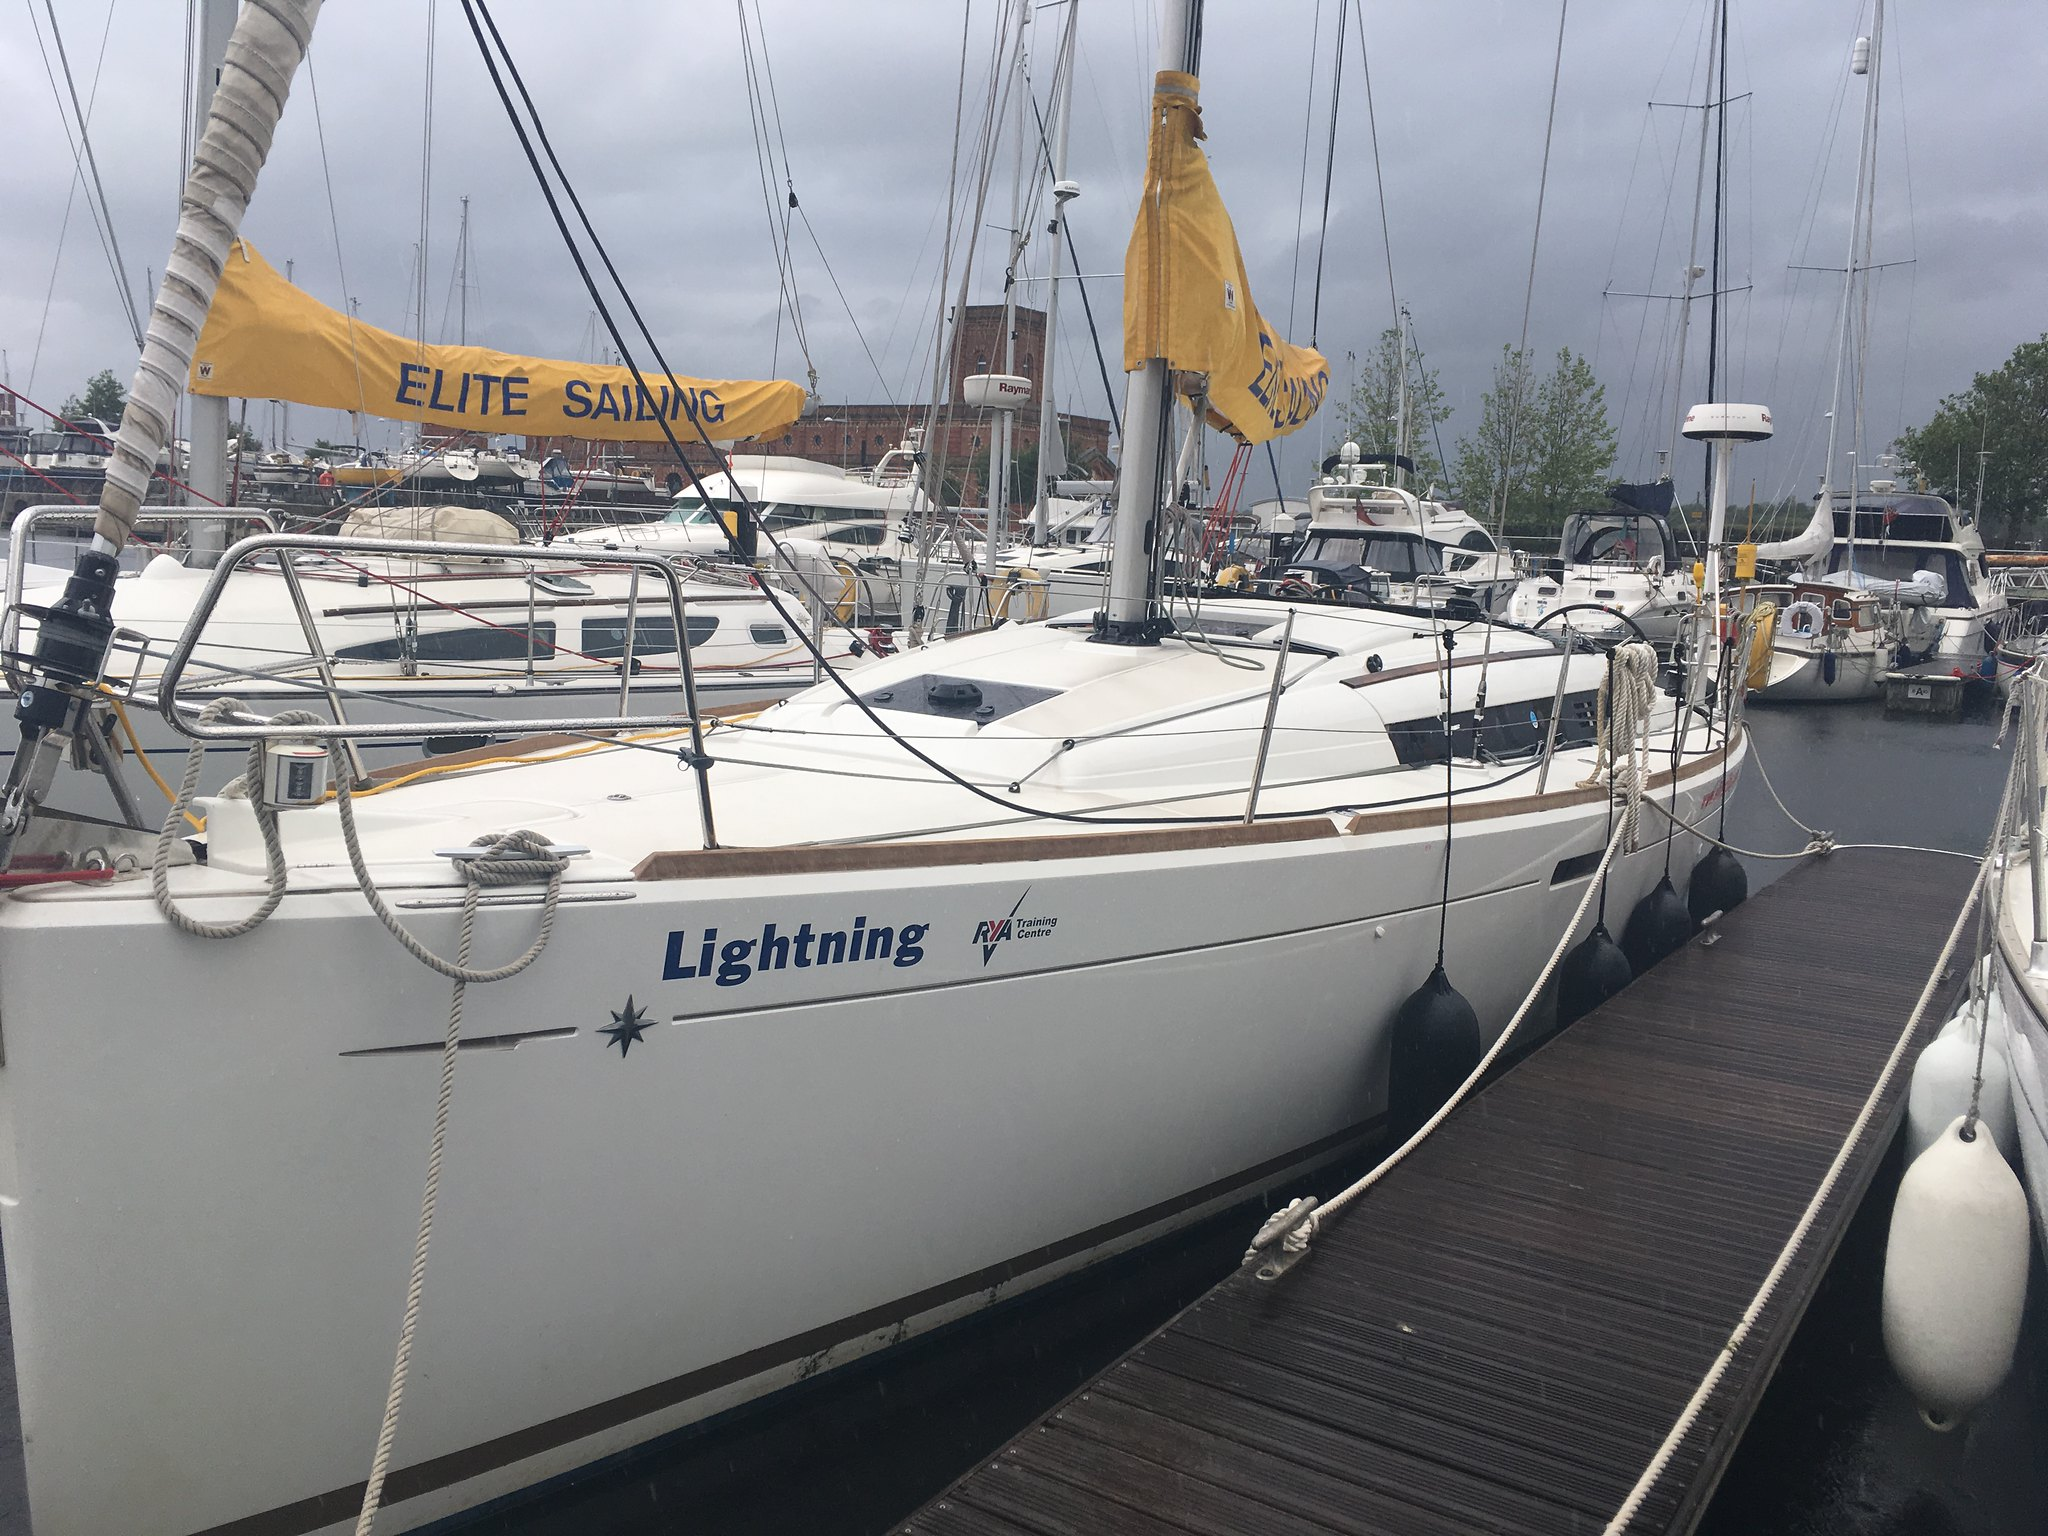
\includegraphics[width=8cm]{art/image1}};
\begin{Large}
\node[anchor=center] at (5,5) {My Title};
\end{Large}
\begin{large}
\node[anchor=center] at (5,4) {- My Subtitle -};
\end{large}
\node[anchor=center] at (5,3) {2023};
\end{tikzpicture}
\newpage

\begin{tikzpicture}[remember picture,overlay,shift={(current page.south west)}]
\begin{normalsize}
\node[anchor=center,align=left] at (5,8) {
First page information: \\
\\
- Item 1 \\
- Item 2 \\
- Item 3
};
\end{normalsize}
\end{tikzpicture}
\newpage

% The Table of Contents
\tback
\tableofcontents
\thispagestyle{empty}
\newpage
\tback
\mbox{}
\newpage
\pagenumbering{arabic}


\section{A CHAPTER}
\subsection{A Section}
\rback{MyColor1}

Sed ut perspiciatis unde omnis iste natus error sit voluptatem accusantium doloremque laudantium, totam rem aperiam, eaque ipsa quae ab illo inventore veritatis et quasi architecto beatae vitae dicta sunt explicabo. Nemo enim ipsam voluptatem quia voluptas sit aspernatur aut odit aut fugit, sed quia consequuntur magni dolores eos qui ratione voluptatem sequi nesciunt.

\begin{small}
\begin{tikzpicture}[remember picture,overlay,shift={(current page.south west)}]
\node[anchor=north west] at (4,5) {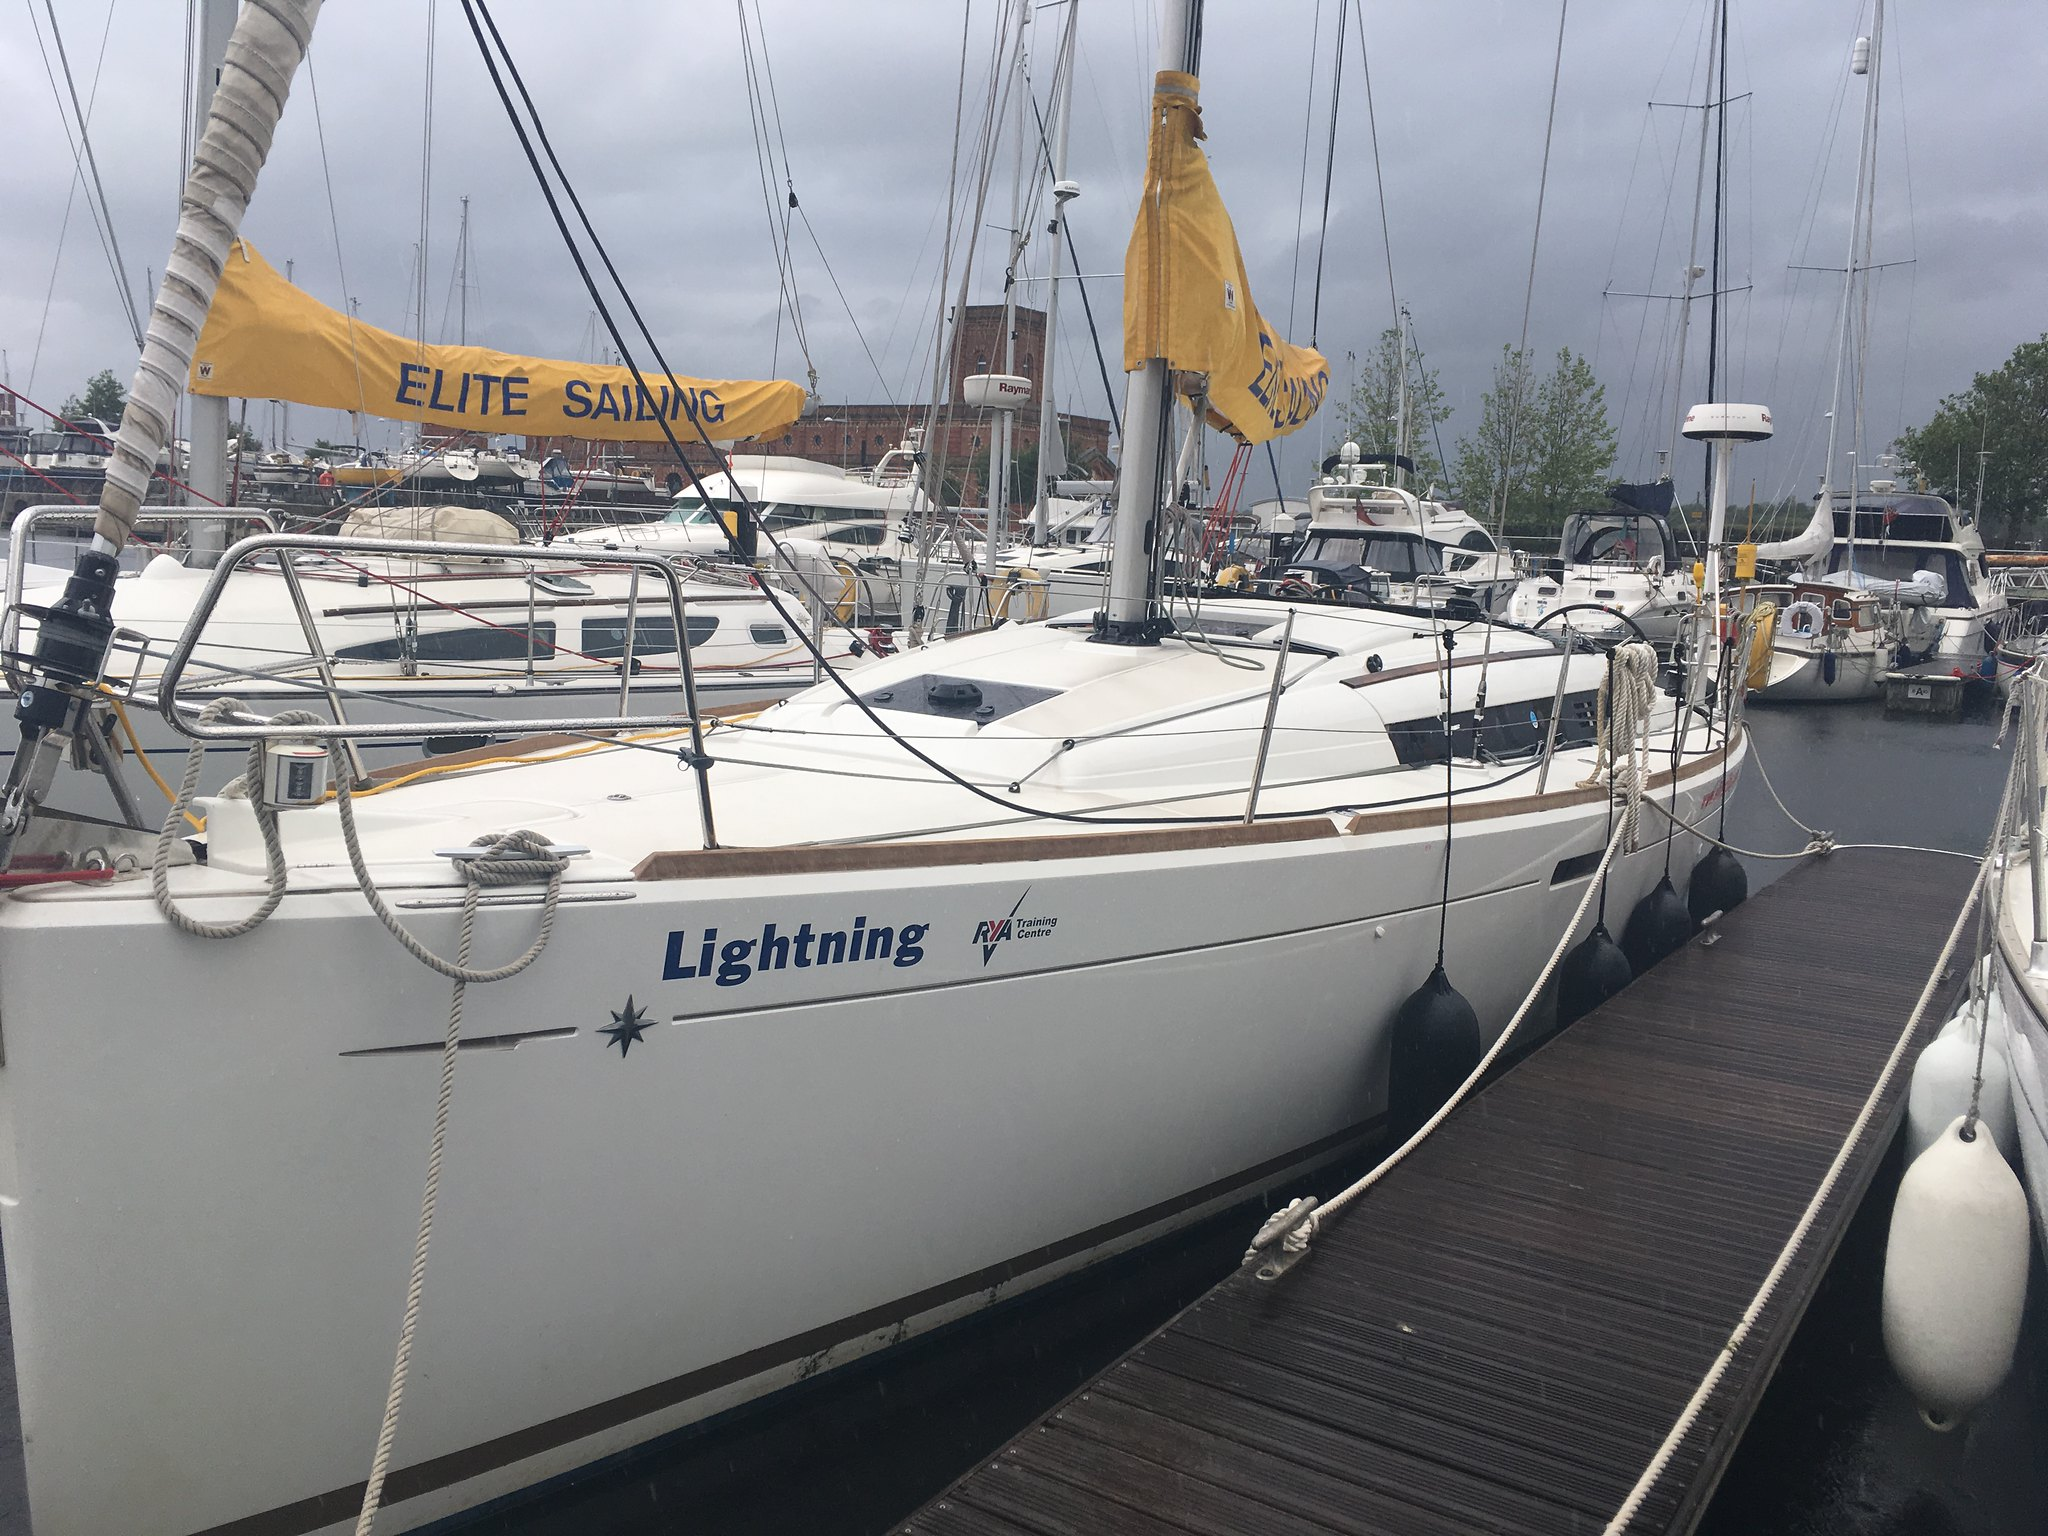
\includegraphics[width=2cm]{art/image1}};
\node[anchor=north west,align=left] at (6.2,4.8) {Manually placed \\ image \\ with caption};
\end{tikzpicture}
\end{small}

Neque porro quisquam est, qui dolorem ipsum quia dolor sit amet, consectetur, adipisci velit, sed quia non numquam eius modi tempora incidunt ut labore et dolore magnam aliquam quaerat voluptatem. Ut enim ad minima veniam, quis nostrum exercitationem ullam corporis suscipit laboriosam, nisi ut aliquid ex ea commodi consequatur? Quis autem vel eum iure reprehenderit qui in ea voluptate velit esse quam nihil molestiae consequatur, vel illum qui dolorem eum fugiat quo voluptas nulla pariatur?


\newpage
\section{ANOTHER CHAPTER}
\subsection{A Different Section}
\lback{MyColor2}

Donec a massa sollicitudin, finibus elit ac, pharetra dolor. Vivamus eget diam mi. In in tellus non nisi euismod dictum. Fusce in accumsan velit. Pellentesque est nulla, luctus tempus ante eu, sagittis congue dolor. Proin sapien dui, condimentum at eros quis, semper ullamcorper leo. Lorem ipsum dolor sit amet, consectetur adipiscing elit. Aliquam dictum nibh sit amet ipsum sodales dapibus. Praesent ornare ante ut aliquam euismod. Vestibulum sodales eros quis sem ullamcorper iaculis. Vivamus sit amet tellus at augue efficitur venenatis. Pellentesque sit amet augue non odio auctor faucibus blandit iaculis neque. Curabitur interdum tempor ante, et varius tellus scelerisque non. Vivamus ut semper massa. Nullam elementum scelerisque felis. Suspendisse est neque, lacinia eget lacus quis, varius tempus ligula.


\newpage
\subsection{A Third Section}
\rback{MyColor3}

Praesent finibus quis purus eu feugiat. Nullam gravida tempor orci id efficitur. Donec ultricies pulvinar consectetur. Lorem ipsum dolor sit amet, consectetur adipiscing elit. Ut eu quam odio. Mauris hendrerit ornare erat vitae posuere. Nunc nec libero ac elit aliquam elementum. Etiam felis risus, sodales eu ornare nec, fermentum feugiat justo. Proin quis sapien purus. Fusce eget augue diam. Maecenas sed venenatis mauris. Ut mattis lectus libero, vitae porta neque scelerisque non. Aenean lacinia vestibulum lectus id ultricies. Donec tempor quis ligula ut vulputate.

\end{document}
